\section{Code-Metriken}
Eine andere Herangehensweise für die werkzeuggestützte Analyse stellt die Ermittlung von \textbf{Code-Metriken} dar.\\
Hierbei werden \textbf{Kennzahlen} bestimmt, anhand derer sich die \textbf{Wartbarkeit} von Source-Code beurteilen lässt.\\
Code-Metriken stehen in \textit{engem Zusammenhang} mit \textbf{Prinzipien guten Entwurfs} (s. Abschnitt~\ref{sec:prinzipien-guten-entwurfs}).\\
Im Folgenden werden die laut \textit{Wedemann} wichtigsten Code-Metriken zur Analyse objektorientierter Software vorgestellt (s. Abbildung~\ref{fig:metriken}).

\begin{figure}
    \centering
    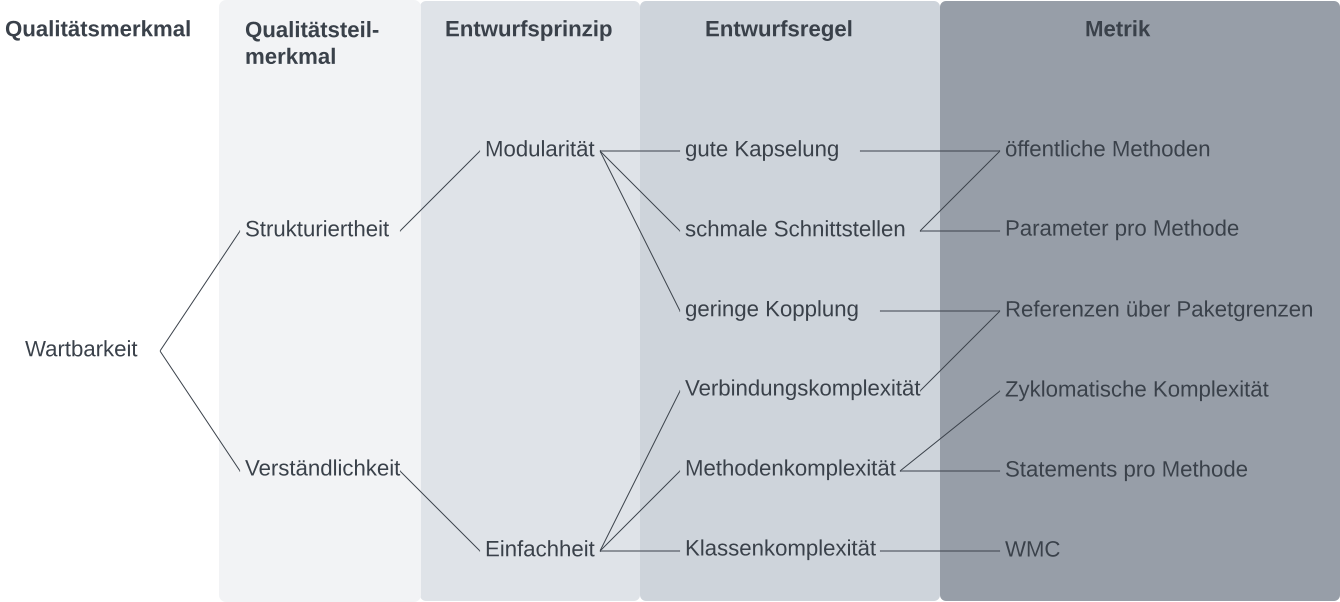
\includegraphics[scale=0.35]{part four/Werkzeuggestützte Analyse/img/metriken}
    \caption{Typische Metriken zur Bestimmung des \textbf{Qualitätsmerkmals} \textit{Wartbarkeit} und ihr Zusammenhang mit den Qualitätsteilmerkmalen. \textbf{WMC} steht für  \textit{Weighted Mean Complexity} (s. ``Komplexität``). (Quelle: in Anlehnung an \cite[Abb. 4.3, 37]{Wed09c})}
    \label{fig:metriken}
\end{figure}

\begin{tcolorbox}[colback=white]
    \textbf{Wartbarkeit} von Code ist immer auch abhängig von den Qualitätsteilmerkmalen \textbf{Strukturiertheit} und \textbf{Verständlichkeit}, die sich mit Metriken messen lassen.
\end{tcolorbox}
\vspace{2mm}

\noindent
Folgende Qualitätsteilmerkmale werden erfüllt, wenn der Entwurf bestimmte Regeln bzw. Prinzipien befolgt, die sich dann in der Implementierung widerspiegeln:

\begin{itemize}
    \item gut strukturierter Code ist leichter zu ändern
    \item einfach zu verstehender Code lässt sich leichter ändern
\end{itemize}

\begin{tcolorbox}
    Ob die Qualitätsforderung \textbf{Wartbarkeit} erreicht ist, kann auch durch Code-Metriken überprüft werden, die versuchen, Prinzipien wie \textbf{Modularität} und Regeln wie \textbf{geringe Kopplung} in Zahlen zu fassen (vgl.~\cite[38]{Wed09c}).
\end{tcolorbox}
\vspace{2mm}

\subsection*{Modularität}
Wenn Quellcode \textbf{modular} ist, ist er auch \textbf{gut strukturiert}.\\
Zur Messing von \textbf{Modularität} werden Metriken zu 3 \textbf{Entwurfsregeln} betrachtet:

\begin{enumerate}
    \item \textbf{gute Kapselung} entsteht durch \textit{wenige} \textbf{öffentliche Methoden}
    \item \textbf{schmale Schnittstellen} bewirkt eine \textbf{niedrige Kopplung}: Dies wird insgesamt erreicht durch \textit{wenig öffentliche Methoden} mit einer \textit{geringen Anzahl von Parametern}\footnote{
    s. auch \textit{Data Coupling}, Abschnitt~\ref{subsec:lose-kopplung}
    }
    \item \textbf{geringe Kopplung von Paketen} wird erreicht, indem wenige Referenzen über Paketgrenzen hinausgehen.
\end{enumerate}


\subsection*{Zyklomatische Zahl}
Zur Abschätzung der \textbf{Komplexität einer Methode} wird häufig die \textbf{zyklomatische Zahl} (auch: \textit{McCabe-Metrik}\footnote{
s. \url{https://de.wikipedia.org/wiki/McCabe-Metrik}, abgerufen 25.05.2024
}) verwendet.\\
Sie gibt die Anzahl unabhängiger Zyklen an, also die Anzahl der Verzweigungen in einer Methode $+1$.\\
Formal lässt sich die \textbf{zyklomatische Zahl} aus dem \textbf{Kontrollflussgraphen} bestimmen: Mit $n$ als Anzahl der Knoten und $e$ als Anzahl der Kanten berechnet sich die zyklomatische Zahl zu $Z = e - n + 2$.\\
Ist eine zyklomatische Zahl hoch, wird von einer hohen Komplexität ausgegangen.\\
Als Beispiel sei nochmals der Kontrollflussgraph zu der Methode \code{countVowels()}\footnote{
    s. Abschnitt~\ref{sec:hilfsmittel-kontrollflussgraph}
} gegeben (s. Abbildung~\ref{fig:zyklomatischezahl}):  Mit $n = 8$ und $e = 9$ berechnet sich die zyklomatische Zahl zu $e - n + 2 = 9 - 8 + 2 = 3$


\begin{figure}
    \centering
    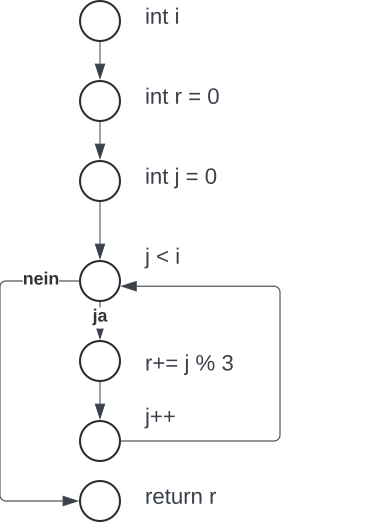
\includegraphics[scale=0.4]{part four/Werkzeuggestützte Analyse/img/kontrollflussgraph}
    \caption{Kontrollflussgraph für \textit{countVowels()}, für den sich eine zyklomatische Zahl von $Z=3$ ergibt. (Quelle: in Anlehnung an \cite[Abb. 4.1, 32]{Wed09c})}
    \label{fig:zyklomatischezahl}
\end{figure}

\noindent
\textit{Wedemann} merkt an, dass die zyklomatische Zahl von zwei \textit{verschachtelten} Schleifen oder Bedingungen genauso groß sei wie die von zwei aufeinanderfolgenden Schleifen oder Bedingungen, obwohl verschachtelte Konstrukte meist schwerer verständlich sind, und dass eine zyklomatische Zahl von $>10$ von vielen Autoren als problematisch betrachtet wird\footnote{
McCabe verwendet in seinem Paper $10$ als ``a reasonable, but not magical,  upper limit.`` (\cite[314]{McC76})
} (vgl.~\cite[38]{Wed09c}).


\subsection*{Komplexität}
Ein weiteres Maß für die \textbf{Komplexität einer Methode} ist die \textbf{Anzahl der Anweisungen}\footnote{auch: Anzahl der Zeilen. Eine Anweisung kann über mehrere Zeilen gehen.}.
Lange Methoden sind sicherlich schwieriger zu verstehen, weshalb auch hier weniger Anweisungen besser sind.\\
Die \textbf{Komplexität einer Klasse} kann mit Hilfe der \textbf{Weighted Mean Complexity} (\textit{WMC}) gemessen werden, für deren Bestimmung die zyklomatische Zahlen \textit{aller Methoden} zusammengezählt werden - auch hier ist ein geringerer Wert besser.

\subsection*{Vorgehen}
Für den Umgang mit den berechneten Zahlenwerten gibt es zwei Strategien:

\begin{enumerate}
    \item Zu den verschiedenen Metriken sind in der Literatur oder den Werkzeugen typische Grenzen angegeben, innerhalb derer Code als ``gut`` betrachtet werden kann.
    \item Da die in (1) erwähnten Grenzen willkürlich erscheinen können bzw. sich verschiedene Quellen bei der Angabe der Grenzen widersprechen können, werden Projekte oft mit einem Satz von Standardwerten untersucht und dann ggf. an das Projekt angepasst.
\end{enumerate}

\noindent
Werden Metriken in einem bereits fortgeschrittenen Projekt eingesetzt, sollten nur die Klassen und Methoden untersucht werden, die besonders auffällig sind.

\subsection*{Werkzeuge}
Für Java gibt es bspw. \textit{Metrics}\footnote{
\url{https://metrics.dropwizard.io}, abgerufen 25.05.2024
}, für PHP bspw. \textit{PHPMetrics}\footnote{
    \url{https://www.phpmetrics.org}, abgerufen 25.05.2024
}.

\subsection*{Pro und Contra}
Code-Metriken sind ein bewährtes Mittel zur Analyse von Code in Bezug auf \textbf{Wartbarkeit}.\\
Wenn Metriken parallel zur laufenden Entwicklung eingesetzt werden, können viele Schwachstellen vermieden werden - sie sind allerdings auch geeignet, um in fremden Code Schwachstellen zu entdecken, wodurch sie ein wertvolles Werkzeug für Projektleiter, QS-Verantwortliche und auch Kunden sind (vgl.~\cite[39]{Wed09c}).\\
In der Praxis kann es sich als schwierig erweisen, geeignete Metriken auszuwählen und die ermittelten Daten korrekt zu interpretieren: Hier werden fehlerhafte Ergebnisse dann durch ungeeignete oder falsch interpretierte Metriken verursacht, was zu Ablehnung der Werkzeuge führen kann.\\
Es ist also ratsam, sich in die einzusetzenden Metriken einzuarbeiten und an bekannten Projekten zunächst auszuprobieren.
